% Base sur la VO 0.11.9
% Relecture technique: 
% Relecture syntaxique: 

\part{Phase de tir}

Lors de la \emph{Phase de Tir}, les figurines équipées d'armes de tir peuvent les utiliser.

\section{Étapes de la phase de tir}

La \emph{Phase de Tir} est divisée en quatre étapes. Suivez l'ordre de la table \ref{table/etapes_tir}.

\begin{table}[!htbp]
\centering
\begin{tabular}{c|m{12cm}}
\textbf{1} & Début de la \emph{Phase de Tir}. \tabularnewline
\textbf{2} & Choisissez une unité avec laquelle tirer. Tirez ! \tabularnewline
\textbf{3} & Retournez à l'étape 2. Choisissez à chaque fois une nouvelle unité qui n'a pas tiré lors de cette phase. \tabularnewline
\textbf{4} & Quand toutes les unités pouvant tirer et que vous souhaitez faire tirer ont tiré, la \emph{Phase de Tir} prend fin. \tabularnewline
\end{tabular}
\caption{\label{table/etapes_tir}Étapes de la phase de tir.}
\end{table}

\subsection{Comment tirer}

Chaque unité équipée d'armes de tir peut tirer une fois par \emph{Phase de Tir}. Les unités en fuite, engagées au corps à corps, qui ont fait une \emph{Marche Forcée}, une \emph{Reformation}, qui se sont ralliées ou qui ont déclaré une charge lors de la \emph{Phase de Mouvement} de ce tour ne peuvent pas tirer.

Quand une unité veut tirer, commencez par nommer une cible dans le champ de vision de l'unité. Il est interdit de tirer sur des unités engagées au corps à corps. Toutes les figurines d'une même unité tirent sur la même cible. Seules les figurines du premier et du deuxième rang peuvent tirer. Si elles possèdent plusieurs armes de tir, annoncez quelle arme est utilisée. Les figurines ordinaires doivent toutes utiliser la même, tandis que les \emph{Champions} et \emph{Personnages} peuvent choisir séparément. Chaque figurine de l'unité est libre de décider de ne pas tirer.

Vérifiez la ligne de vue de chaque figurine. Souvenez-vous que la ligne de vue est toujours tracée depuis l'avant. Les figurines qui n'ont pas de ligne de vue sur la cible ne peuvent pas tirer. Vérifiez la portée du tir pour chaque figurine qui tire. La portée est mesurée depuis chaque figurine jusqu'au point le plus proche de l'unité cible, même si ce point n'est pas dans la ligne de vue. Les figurines hors de portée ne peuvent pas tirer. Une fois que vous avez déterminé les figurines pouvant tirer, lancez les jets pour toucher pour celles-ci.

\section{Jets de dé pour toucher}

Quand vous lancez le jet pour toucher, utilisez la Capacité de Tir (CT) de la figurine qui tire. Si la figurine a plusieurs profils, comme par exemple un cavalier et sa monture, utilisez la CT de l'élément qui tire. 

\subsection{Modificateurs au jet pour toucher}
\label{tir/modificateurs}

Les attaques de tir peuvent subir un ou plusieurs modificateurs sur leurs jets pour toucher. Additionnez simplement les modificateurs à la CT du tireur. La liste de ce paragraphe décrit les modificateurs usuels, mais les sorts et capacités peuvent ajouter d'autres modificateurs. Si les modificateurs provoquent des résultats de 7+, 8+ ou 9+, lancez les jets comme décrit dans la table \ref{table/tir_pour_toucher}. La table \ref{table/modificateur_tir} résume les modificateurs.

Le joueur contrôlant l'unité qui tente de toucher jette un dé par figurine. Si le résultat est supérieur ou égal à \result{7 moins la CT} de la figurine, le tir touche sa cible. Un résultat de \result{1} est toujours un échec. La table \ref{table/tir_pour_toucher} référence les résultats nécessaires pour toucher.

Si au moins un tir a touché, suivez la procédure décrite dans la section \ref{attaque_et_blessure} à la page \pageref{attaque_et_blessure}.

\renewcommand{\arraystretch}{1.2}
\begin{table}[!htbp]
\centering
\begin{tabular}{r|c}
Longue portée & -1 \\
Bouger et tirer & -1 \\
Tenir la position et tirer & -1 \\
Couvert léger & -1 \\
Couvert lourd & -2 \\
\end{tabular}
\caption{\label{table/modificateur_tir}Modificateurs au jet pour toucher.}
\end{table}
\renewcommand{\arraystretch}{1.5}

\renewcommand{\arraystretch}{1.2}
\begin{table}[!htbp]
\centering
\begin{tabular}{cc}
\hline
\textbf{CT avec modif.} & \textbf{Résultat nécessaire} \\
\hline
6 ou plus & 2+ \\
5 & 2+ \\
4 & 3+ \\
3 & 4+ \\
2 & 5+ \\
1 & \result{6} \\
0 & \result{6} suivi par 4+ \\
-1 & \result{6} suivi par 5+ \\
-2 & \result{6} suivi d'un \result{6} \\
-3 ou moins & impossible \\
\hline
\end{tabular}
\caption{\label{table/tir_pour_toucher}Jets pour toucher (tir).}
\end{table}
\renewcommand{\arraystretch}{1.5}



\subsubsection*{Longue portée}

\textbf{-1 pour toucher}

Si la figurine se trouve au-delà de la moitié de la portée de l'arme, la figurine qui tire subit un modificateur pour toucher de -1. Souvenez-vous que la portée doit être vérifiée pour chaque figurine individuellement.

\subsubsection*{Bouger et tirer}

\textbf{-1 pour toucher}

Si l'unité s'est déplacée lors de ce tour du joueur, chaque figurine subit un modificateur pour toucher de -1.

\subsubsection*{Tenir la position et tirer}

\textbf{-1 pour toucher}

Les attaques de tir réalisées pendant la réaction à la charge \emph{Tenir la Position et Tirer} ont un modificateur pour toucher de -1.

\subsubsection*{Couvert}

\textbf{-1 ou -2 pour toucher}

Le couvert est déterminé individuellement, pour chaque figurine de l'unité qui tire. Il existe deux types de couvert, \emph{Léger} ou \emph{Lourd}. Dans les deux cas, le couvert est déterminé en utilisant la ligne de vue de la figurine qui tire. Tracez des lignes de vue depuis un point au choix à l'avant du socle de la figurine jusqu'à tout point de l'empreinte au sol de l'unité visée, sachant que dans le cadre des couverts, la ligne de vue peut sortir de l'arc frontal. Si ces lignes passent par un terrain, un décor ou une figurine, le tireur aura un malus pour toucher dépendant du type de figurine, de terrain, de décor et du nombre de lignes de vue interceptées. Les figurines ignorent toujours les figurines de leur propre unité ou de l'unité ciblée pour la détermination du couvert.

\subsubsection*{Cible derrière un couvert léger}

Une figurine tirant sur une cible derrière un \emph{Couvert Léger} subit un modificateur pour toucher de -1. Le \emph{Couvert Léger} s'applique si au moins la moitié de l'empreinte au sol de l'unité ciblée est cachée par un ou plusieurs des éléments suivants (voir figure \ref{figure/couvert_leger}) :
\begin{itemize}[label={-}]
\item Terrain offrant un \emph{Couvert Léger}.
\item \nouveau{Figurines, de n'importe quelle taille. Si vous tirez avec ou sur des figurines de \emph{Grande Taille} (voir le paragraphe \ref{hauteur_figs} à la page \pageref{hauteur_figs}), ignorez les figurines de \emph{Petite Taille} pour déterminer s'il y a un \emph{Couvert Léger}.}
\end{itemize}

\subsubsection*{Cible derrière un couvert lourd}

Une figurine tirant sur une cible derrière un \emph{Couvert Lourd} subit un modificateur pour toucher de -2. Si une cible est à la fois derrière un \emph{Couvert Léger} et un \emph{Couvert Lourd}, n'appliquez que la pénalité de \emph{Couvert Lourd}. Le \emph{Couvert Lourd} s'applique si au moins la moitié de l'empreinte au sol de l'unité visée est cachée par un ou plusieurs des éléments suivants (voir figure \ref{figure/couvert_lourd}) :
\begin{itemize}[label={-}]
\item Terrain offrant un \emph{Couvert Lourd}.
\item Figurines de la même \emph{Taille} ou plus grandes que le tireur \textbf{et} sa cible (voir le paragraphe \ref{hauteur_figs} à la page \pageref{hauteur_figs}).
\end{itemize}

\subsubsection*{Cible derrière un couvert léger et un couvert lourd}

Si l'empreinte au sol de l'unité visée est cachée à la fois par des éléments pouvant offrir un \emph{Couvert Léger} et un \emph{Couvert Lourd}, mais pas assez pour obtenir l'un ou l'autre des couverts, le tireur subit la pénalité de \emph{Couvert Léger} si au moins la moitié de l'empreinte au sol de l'unité visée est cachée par l'ensemble des éléments (voir figure \ref{figure/couvert_leger_et_lourd}). Par exemple, si la cible est cachée à 30 \% par des éléments offrant un \emph{Couvert Léger} et à 30 \% par des éléments offrant un \emph{Couvert Lourd}, le tireur subit la pénalité du \emph{Couvert Léger}.

\begin{figure}[!htbp]
\centering
\def\svgwidth{\columnwidth}
\input{couvert_leger.pdf_tex}
\caption{a) Ces figurines ne peuvent pas tirer, car l'ennemi est hors de leur champ de vision. \\
b) Ces figurines peuvent tirer, l'ennemi est dans leur champ de vision, et aucun couvert n'est pris en compte car moins de la moitié de l'empreinte au sol de l'unité visée est cachée par la \emph{Forêt}. \\
c) Ces figurines peuvent tirer, mais souffrent de la pénalité de \emph{Couvert Léger}, car plus de la moitié de l'empreinte au sol de l'unité visée est cachée par la \emph{Forêt}.}
\label{figure/couvert_leger}
\end{figure}

\begin{figure}[!htbp]
\centering
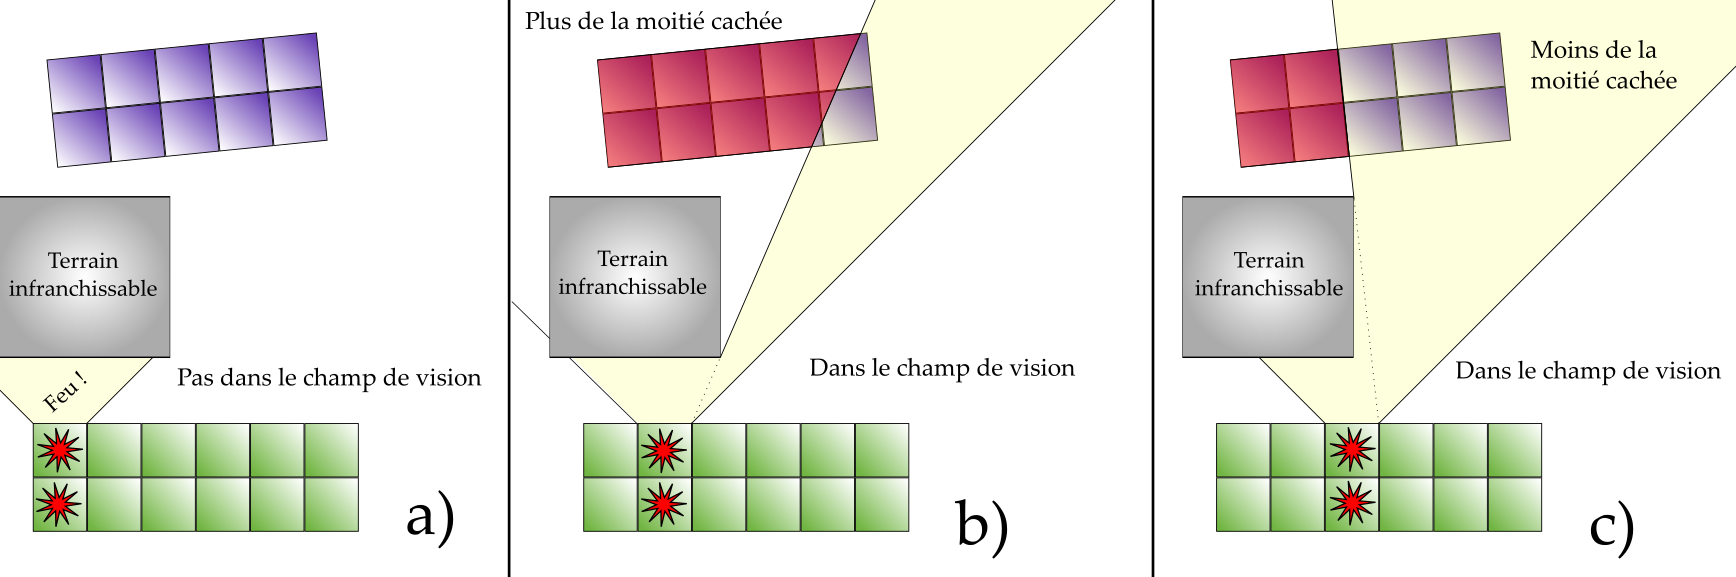
\includegraphics[width=15.5cm]{couvert_lourd.png}
\caption{a) Ces figurines ne peuvent pas tirer, car l'ennemi est hors de leur champ de vision. \\
b) Ces figurines peuvent tirer, mais souffrent de la pénalité de \emph{Couvert Lourd}, car plus de la moitié de l'empreinte au sol de l'unité visée est cachée par le \emph{Terrain Infranchissable}. \\
c) Ces figurines peuvent tirer, et aucun couvert n'est pris en compte car moins de la moitié de l'empreinte au sol de l'unité visée est cachée par le \emph{Terrain Infranchissable}.}
\label{figure/couvert_lourd}
\end{figure}

\newpage

\begin{figure}[!htbp]
\centering
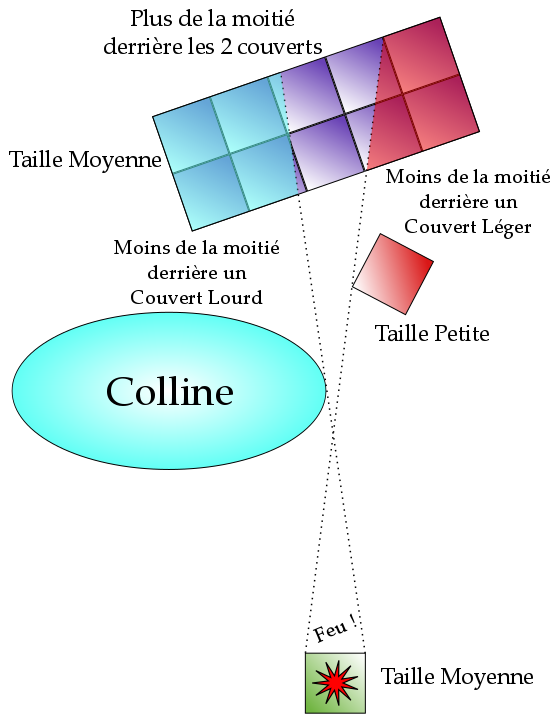
\includegraphics[width=6cm]{couvert_leger_et_lourd.png}
\caption{Dans cet exemple, moins de la moitié de l'empreinte au sol de la cible est cachée par un \emph{Couvert Léger} ou un \emph{Couvert Lourd}. Toutefois la combinaison des deux en cache plus de la moitié, donc la cible compte comme étant derrière un \emph{Couvert Léger}.}
\label{figure/couvert_leger_et_lourd}
\end{figure}

\subsection{Lignes de vues et couverts}

Ce schéma résume les cas les plus communs pour déterminer des lignes de vues et des couverts entre une figurine avec des attaques à distance, une figurine occultante et sa cible (en fonction de la taille de la figurine).
\begin{figure}[!htbp]
\centering
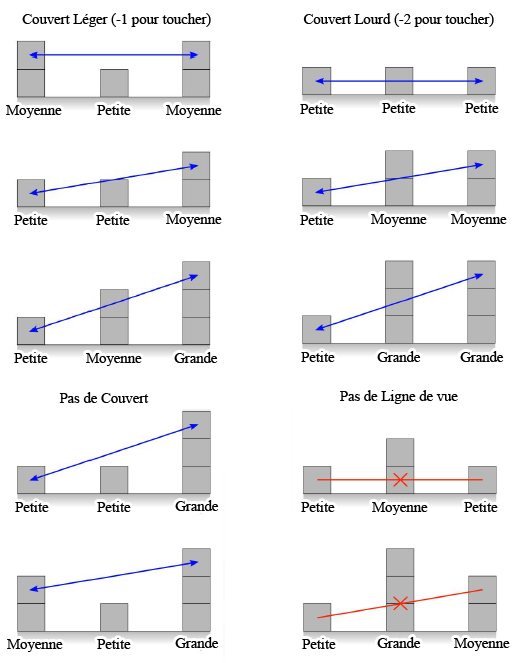
\includegraphics[width=12cm]{Lignes_de_vue.png}
\end{figure}

